%
% File hicss51.tex
%
% Contact: Holm Smidt, hsmidt@hawaii.edu
%%
%%
%% Based on the style files for ACL 2015 by 
%% car@ir.hit.edu.cn, gdzhou@suda.edu.cn


\documentclass[10pt]{article}
\usepackage[letterpaper]{geometry}
\usepackage{hicss51}
\usepackage{times}
\usepackage[none]{hyphenat}
\usepackage{url}
\usepackage{latexsym}
\usepackage{minted}
\usepackage{indentfirst}
\usepackage{graphicx}
\graphicspath{{images/}}

\usepackage{blindtext}
\usepackage{amsmath}
\usepackage{eurosym}
\newcommand{\sansserifformat}[1]{\fontfamily{cmss}{ #1}}%

%\setlength\titlebox{5cm}

% You can expand the titlebox if you need extra space
% to show all the authors. Please do not make the titlebox
% smaller than 5cm (the original size).


\title{Improving Waste Collection Procedures \\ In Practical Smart City Implementations}

\author{
  Jan D{\"u}nnweber  \\
  Ostbayerische Technische \\ Hochschule Regensburg \\
  {\underline{ jan.duennweber@othr.de} }\\\And 
  Amitrajit Sarkar \\
 Ara Institute \\ of Canterbury \\
  {\underline{amit.sarkar@ara.ac.nz}} \\\And
  Vimal Kumar Puthiyadath \\
 KPIT Technologies Ltd \\
  {\underline{Vimal.Puthiyadath@kpit.com}} 
  }

\date{}

\begin{document}
\maketitle
\begin{abstract}
Computer-based Improvements to waste collection procedures are often a part of smart city 
initiatives. When we envision an ideal waste collection vehicle, it will arrive at every
container exactly at the time when it is fully loaded. Beyond doubt, this will 
reduce traffic and support environmentally friendly intentions like an expansion 
of waste separation as it will make more containers manageable. 
An obvious difficulty of putting that vision into practice is that  
collection vehicles cannot always be where they are needed. 
Knowing the best time for emptying a container is insufficient for 
finding the optimal collection route.
Therefore, we compare three different approaches to reducing the waste collection
times by the use of networked fill-level sensors: Regensburg,
Christchurch and Pune. Our analysis shows that the most efficient collection schedules 
result from adapting field-tested routes frequently on the basis of 
current sensor measurements and shortcuts resulting from route 
optimization computations.
\end{abstract}

\section{Introduction}
Even with the latest IoT technology like networked sensors and simulations
forecasting the collection times of megacities, practical implementations of 
on-demand waste collection still have difficulties in keeping up with the 
prognosticated improvements.
A collection vehicle that drives obstinately from the most heavily filled 
container to one with the fill-grade closest to that will obviously need 
more time in the majority of cases than a vehicle following a fixed plan, 
since heavily filled containers are probably positioned far apart from 
each other. Finding a smarter route leads us to the classic 
{\it vehicle routing problem} (VRP~\cite{Dantzig59}), an instance of the 
{\it Travelling Salesman Problem (TSP)} with the added constraint that we 
need to return to the starting point after visiting a fixed number of points, 
since the collection vehicle has a limited capacity. 
Thus, we don't need to find the minimum Hamiltonian
circle through all the points but multiple circles forming some kind of
clover leaf. However, finding the best route to collect the waste 
containers does not only require to consider the distances between 
the single containers. Containers which are only filled to a certain level should
be skipped, i.\,e. we are dealing with a instance of a dynamic route 
planning problem, which is also the subject of more recent 
research~\cite{Chen16}.

There are $\frac{n!}{2}$ different routes connecting $n$ containers. 
For comparing all routes between only $10$ containers, this means 
3628800 routes must be analyzed. Modern waste collection
vehicles can be loaded with $\approx 400$ container of 120 
liters~\cite{hyundai18}.
$400!$ is a $882$-digit number. Taken into account that skipping 
containers with little load, means the vehicle has to pickup an other
one where it usually does not drive to, solving our dynamic VRP requires
to solve a new problem of that size, every time when the fill-level
measurements are updated. Nowadays, supercomputers can deal with 
such problem sizes~\cite{Burkhovetskiy2017}. However, the
presented projects deal with approximate solutions, which
can be found using a standard PC or an on-board computer in
the garbage truck. Therefore, the presented work might be relevant 
for automating the navigation of future self-driving garbage 
trucks, like the one Volvo started testing in Brussels 
recently~\cite{volvo17}.

The approximate solutions presented in this paper are based on 
the {\it ant colony optimization} (ACO~\cite{Dorigo97}). This 
approach has been proven suitable for dynamic VRP instances
in a simulation, where the road network and the related 
traffic were taken into account~\cite{Karadimas2008}. ACO is a {\it swarm intelligence}
procedure, i.\,e. not an individual (a simulated ant in the case of 
ACO) solves a problem but a group. For finding optimal routes,
the simulation starts with letting the ants take random paths
until they reach their destination. This random walk is optimized
iteratively: each ant leaves a pheromone trail behind it which
evaporates after a certain number of iterations. In every iteration
the pheromone intensity of the shorter paths increases because
whenever a simulated ant can choose among multiple paths, it takes
the one with the highest pheromone intensity. This means, in higher
iterations, the paths are no more randomly chosen but influenced 
by the most successful ants from preceding iterations, which are
the ones whose pheromone trails did not evaporate until their 
followers reached them, since they were on the shortest paths.

The rest of this paper is structured as follows: 
Section~\ref{sec:Regensburg} shows how the city of Regensburg benefits from using 
fill-level sensing and ACO-based route optimization for collecting their biological
waste containers. 
Section~\ref{sec:Christchurch} introduces {\it LevelSense} in Christchurch, 
an IoT-based approach to on-demand waste collection, which also uses ACO and is a 
part of a larger {\it Smart City} initiative in New Zealand, the {\it PiP-IOT project}. 
Section~\ref{sec:Pune} introduces another route optimization algorithm, which is used
by {\tt kpit.com} for solving a related problem: Getting all the employees
from various places in Pune to their their offices. 

Section~\ref{sec:concl} looks back on the three projects, which were all 
put into practice, discusses the {\it lessons learned} from these projects,
their benefits and points out some future perspectives.


\section{The Collection of Biological Waste in Regensburg}
\label{sec:Regensburg}

Our work in Regensburg focuses on improving the collection of biological waste~\cite{Burger18}.
While other approaches toward the computer-aided routing of waste collection vehicles 
rely only on fill-level sensing~\cite{LundinOS17} or only on ACO-based path 
computations~\cite{ismail09}, we combined both ideas. 

\begin{figure}[h!]
  % Use the relevant command to insert your figure file.
  % For example, with the graphicx package use
    \centering
  \includegraphics[trim={3cm 4cm 3cm 3cm}, clip,width=0.5\linewidth]{biobin}
  % figure caption is below the figure
  \caption{Biological Waste Container equipped with a fill-level sensor on the back}
  \label{fig:container}       % Give a unique label
\end{figure}

Simulations have shown, that 
the combination of these techniques can significantly reduce the time needs for the collection
of waste~\cite{Sharmin16}. Since the present contracts with service providers or logistical
obstacles often conflict with changes to the waste collection routes, possible time savings can be 
computed but not really be exploited in many places.
Contrarily, in Regensburg, we recently started applying route optimization and fill-level 
sensing to the collection of the containers for biological waste.
Figure~\ref{fig:container} shows one such container and the protection casing on the
back which houses the electronics (shown in Figure~\ref{fig:electronics}) which we attached 
to it for monitoring the fill level.

\begin{figure}[h!]
  % Use the relevant command to insert your figure file.
  % For example, with the graphicx package use
    \centering
  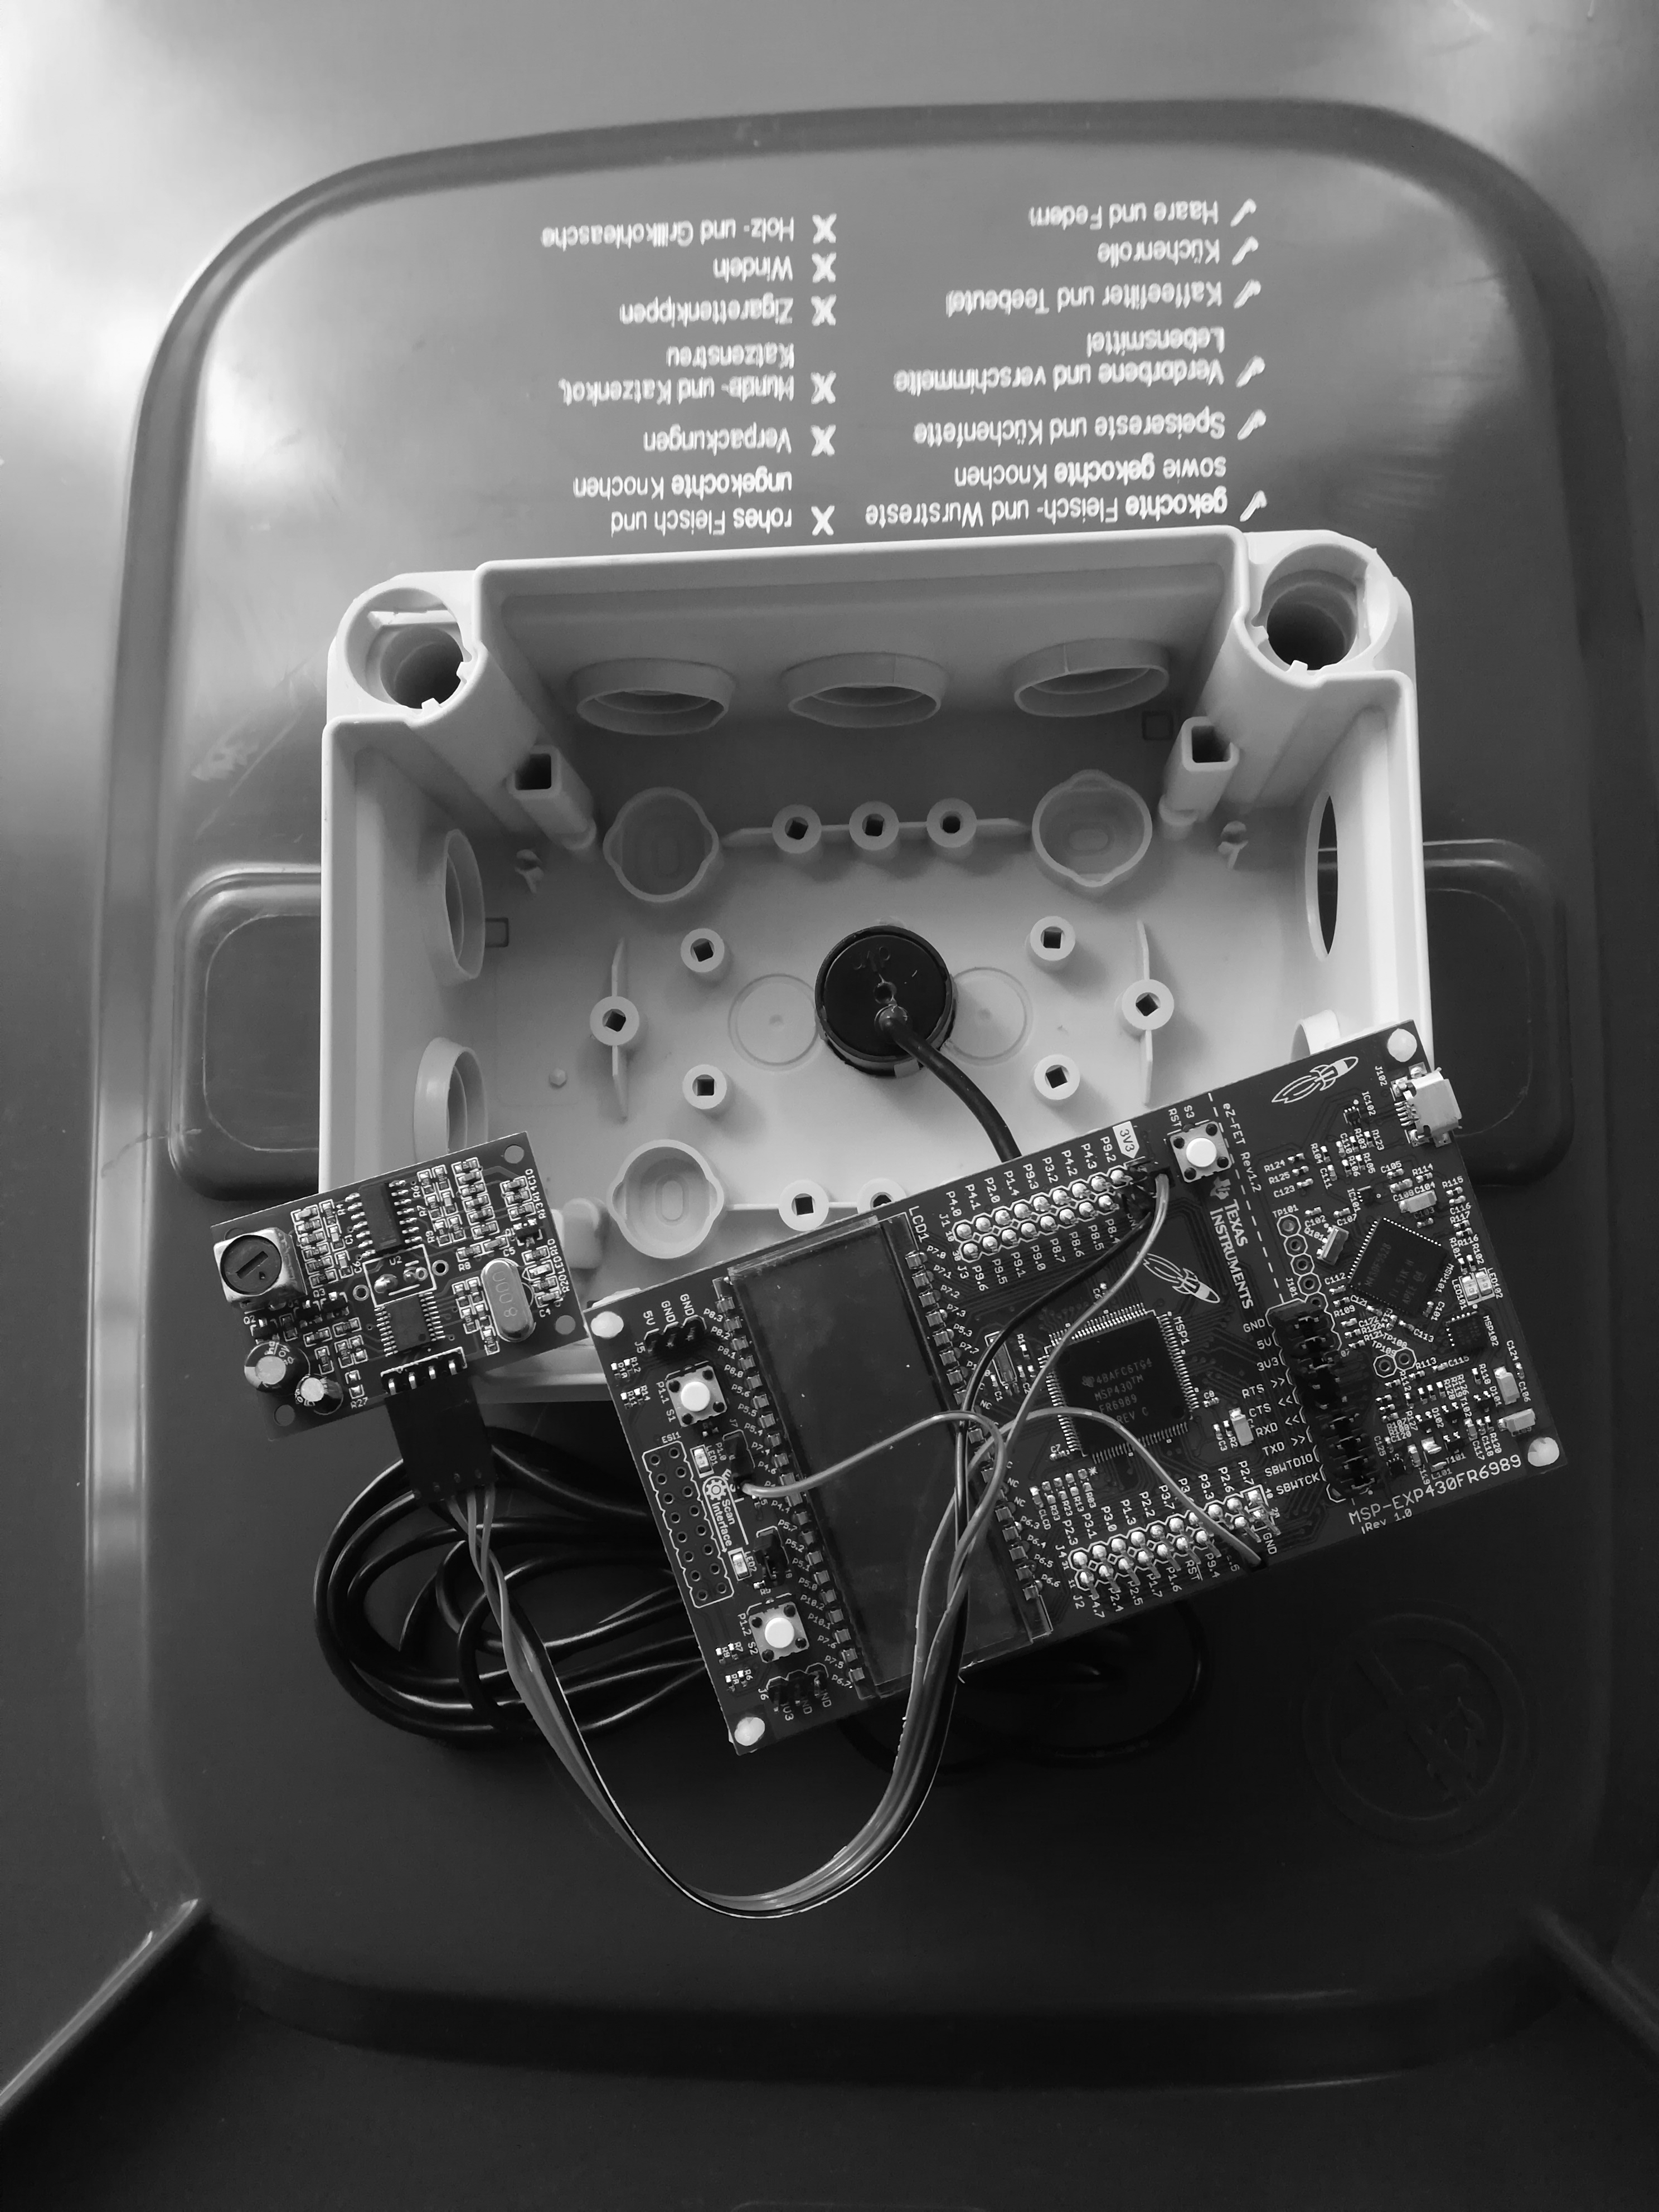
\includegraphics[trim={3cm 4cm 3cm 3cm}, clip,width=0.5\linewidth]{sensor}
  % figure caption is below the figure
  \caption{Detail picture showing the electronics attached to the container}
  \label{fig:electronics}       % Give a unique label
\end{figure}

Regensburg established a novel program for the collection of biological waste in 2018 
and equipped the city and its surrounds with 700 new containers. The novelty of the program
allows us, computer scientists (headed by author Jan D{\"u}nnweber) and electrical 
engineers (headed by his colleague Martin Schubert) at the {\it Technical 
University of Applied Sciences} in Regensburg (OTH), to help forming it.
Noteworthy as well, is that 700 containers are not too many. While the number
of possible thorough paths, connecting all containers is tremendous ($\frac{n!}{2}$ is a 
1719-digit number), there are only  $\tbinom {700}{2}$ ways to choose a interconnecting 
route between an unordered pair of containers, which is 
$\frac{700!}{2!(700 - 2)!}=\frac{700!}{2 \times (698)!}=\frac{699 \times 700}{2}=244650$ interconnections. Combinations vary, but the interconnections are static and can be stored.
Therefore, we set up a database, which holds for half of the 700 containers ({\it one-way})
a file with the distances connecting it to the remaining 699 candidates (244650 entries
totally).

To ascertain the profitability of our undertakings, we also started with a simulation.
However, our simulation did not forecast the profits of ACO on arbitrary routes or the
benefits from observing arbitrary containers. We computed a viable forecast for Regensburg.
With the help of a group of students (David Burger, Vadim Dechand, 
Haris Shehzad and Markus Wildgruber), we could fill the mentioned 
244650-entry database with concrete distances and average driving times. 

After accompanying
the waste collectors and recording the GPS positions of the containers and the time needs 
for emptying them with a fitness tracking app on the smart phone, we requested the
distances for all possible pairs from the {\it Google Maps} Web service by means of a 
Java program, which the students have developed to export the distance data into the
popular TSPLIB-format~\cite{tsplib90}. With this representation, our data can be 
processed using Open-Source ACO-code and other TSP-solvers. Our routing software makes
use of the Thomas St{\"u}tzle Implementation~\cite{Dorigo97} and we used the exact 
TSP-solver {\it Concorde}~\cite{applegate01} as a reference. 


To integrate fill-level sensing into the route computations, started to cope with
underfilled containers. While overfilled containers seem to be 
a more urgent problem, it is difficult (or almost impossible) to send a vehicle  
instantaneously, when an overfilled container is detected. Planning collection 
routes such that underfilled containers are skipped is much easier and saves time.
That saved time is used to collect new containers. The recorded data about
overfilled containers helps to position the new containers where they are needed.
Thus, our waste management software, tackles both problems, underfilled containers directly
(by leaving them our during the collection) and overfilled containers as well, 
by finding the best positions for new containers in the long run. Instead of
resetting the route computations when a container is added, removed or 
re-positioned, we let ACO continuously running, since it is known that the 
swarm algorithm can adapts to its input~\cite{angus2005}.

Master-student Josef Wei{\ss} (from Martin Schubert's group) set up the electronics
shown in Figure~\ref{fig:electronics}: The larger board (on the right) holds an ultrasonic transceiver module and a low power µC. The smaller board (on the left holds) and a 
LoRa (Low Range) transceiver. We communicate the fill grade measured by the 
ultrasonic transceiver via a LoRa gateway. The costs for 10 of this {\it DIY}-devices 
were below $1000$~\EUR{} and sponsored by {\tt kpit.com}.

Using our simulation, we could predict that 10 sensors are enough to start
benefiting from our software. To compute a trustworthy prediction, our simulation
does not simply roll the dice to decide whether a sensor-equipped container can
be skipped. Instead the probability for each container $i$ to be empty was 
computed individually using the formula: $P(x_i)=q_i* \frac{c_i}{d_i}$. The value for 
$q_i$ ranges between $0.1$ (overfull), $0.2$ (full), $0.3$ (half-full) and $0.5$ (empty)
and was set accordingly to the average fill level of that container that we observed on
the collection tours. Parameter $d_i$ takes account for the fact that waste containers 
located near the city center are more likely found full and is set to $1.2$ for a container
withing a $2$ kilometer circle around the center, $1.1$ withing $4$ kilometers and $0.9$ for 
containers located more than $6$ kilometers away from the center. Parameter $c_i$ is weighted 
accordingly to the number of waste containers next to it and set to $0.9$ when there is none or
set to $1.1$ for up to $5$ neighboring containers or set to $1.3$ when there are $6$ or more.
With that estimations, we predicted time savings of approximately one hour per day.
Regensburg has just started to adapt the routes accordingly. Thus, we will soon
know how many extra containers can be emptied within the saved time.

\section{LevelSense and the PiP-IoT project}
\label{sec:Christchurch}

\blindtext

\section{Collecting Employees at {\tt kpit.com}}
\label{sec:Pune}

\blindtext

\section{Conclusion and Future Perspectives}
\label{sec:concl}

\blindtext

% \section{References} 

% List and number all bibliographical references in 9-point Times, single-spaced, at the end of your paper. When referenced in the text, enclose the citation number in square brackets.
% % for example \cite{Jones2015,Smith2015} and \cite{Smith2015}. 
% Where appropriate, include the name(s) of editors of referenced books.

% if added before the last page, this command can help balancing columns
%\addtolength{\textheight}{-.2cm} 

%Bibliography 
\bibliographystyle{ieeetr}
\bibliography{sample}


\end{document}
